\documentclass[conference]{IEEEtran}
\usepackage{cite}
\usepackage{amsmath,amssymb,amsfonts}
\usepackage{algorithmic}
\usepackage{graphicx}
\usepackage{textcomp}
\usepackage{xcolor}
\usepackage{float}
\usepackage{tikz, pgfplots}
\usepackage{circuitikz}
\usepackage[english]{babel}
\usepackage[autostyle, english = american]{csquotes}
\MakeOuterQuote{"}
\def\BibTeX{{\rm B\kern-.05em{\sc i\kern-.025em b}\kern-.08em
    T\kern-.1667em\lower.7ex\hbox{E}\kern-.125emX}}

\pgfplotsset{compat=newest}

\begin{document}

\title{MSP432 Timers, Interrupts, and Analog-to-Digital Converter\\

\author{\IEEEauthorblockN{Tevin Hendess}
\IEEEauthorblockA{\textit{Computer Engineering Department} \\
\textit{Rochester Institute of Technology}\\
Rochester, NY USA \\
twh4619@rit.edu}
\and
\IEEEauthorblockN{Adam Schultzer}
\IEEEauthorblockA{\textit{Computer Engineering Department} \\
\textit{Rochester Institute of Technology}\\
Rochester, NY USA \\
ajs1539@rit.edu}
}
}

\maketitle

\begin{abstract}
An essential part of modern electronics is the ability to interact with
analog voltages that arise from sensors. Important parts of interpreting
these signals are using timers and ADCs (Analog to Digital Converters) to
sample the analog data into digital data. Demonstrating these concepts was
accomplished by enabling the proper peripherals on a MSP432 microcontroller,
these being the ADC and Timer32 modules, and programming the microcontroller
to sample temperature and light sensors, using the Timer32 module
as a clock, and the ADC to receive analog data. Data was processed and
visualized in tests to ensure that the analog sampling was performed as
expected. These tests utilized MatLab to visualize digital conversions,
which were compared to a waveform recorded on an oscilloscope.
\end{abstract}

\section{Design Methodology}

\subsection{Usage of Timers}
In order to accurately sample many external sensors, a clock signal must be 
used to synchronize the outputs of the sensor and the inputs of the ADC in
the microcontroller. Although a clock signal is necessary, the
microcontroller's internal clock would be a poor choice of a signal to use
for this purpose, as inputs would be received at the same pace that the
processor can execute instructions. Instead, timer interrupts were used to
reduce the main clock signal to a significantly slower and more usable
frequency. A Timer32 module of the MSP432 was used for this purpose.

The Timer32 module was used to generate interrupts at a rate of 2Hz and
1kHz, with the 2Hz signal being used to toggle an LED, and the 1kHz signal
being used to measure time between button presses in milliseconds. The 2Hz
signal was also used to trigger data collection from a temperature sensor,
so that the program would receive updated data two times a second.

% part 1 end

\subsection{Analog to Digital Conversion}
Before constructing the final form of the circuit which would take input from a line-scan camera, a more simple ADC circuit was constructed. To practice with analog to digital conversion, a temperature sensor was connected to the MSP432 board via extension wires.

This sensor is much less complicated than a full 128 bit definition camera, but still presented some challenges. The first was pulling the information from the device via the ADC. This required code which would configure one of the ADC clusters on the microcontroller to suit a temperature sensing application. Two of the most important variables that had to be set were the reference voltage (which was set at 2.5V according to information from the MSP432 datasheet) and the interrupts which were completely disabled on the ADC itself.

Though interrupts were used to obtain data from the ADC, the Timer32 module was used as it interrupts at a set frequency rather than the ADC which will interrupt whenever the it receives new data (which would have been far more than required).
Once the raw data from the temperature sensor was converted to a digital value through the ADC hardware, conversions had to be performed, this time in software, to output a human-readable temperature in degrees Centigrade and Fahrenheit. The equation for converting the raw digitized voltage to Celsius is shown in Equation 1.

\begin{equation}
    Celsius = ((int) analogIn) / 142.46f - 10;
\end{equation}

In Equation 1, Celsius is the floating point variable storing the current temperature in degrees Centigrade and analogIn is the direct digitized analog input from the ADC. For these variables, it was very important that the types be correct in order for the mathematical operations to perform as expected. Celsius had to be a floating point value in order to store non-whole numbers and analogIn had to be typecast into an integer rather than used in its original, unsigned integer form. The two constants in Equation 1 come from the temperature sensor datasheet which proclaims a range of the device between 10°C and 125°C. The maximum value was divided by the maximum voltage value of the ADC (3.3V) to determine a scaling factor which was then applied to the analog input. The subtraction of ten accounts for the range offset beginning at 10°C rather than 0°C.

Once the value was expressed in degrees Centigrade, the conversion to Fahrenheit was trivial and is shown in Equation 2.

\begin{equation}
    Fahrenheit = celsius * (9.0f/5.0f) + 32.0f;
\end{equation}

Because the celsius variable is already a floating point value, no special typecasts need to be performed in Equation 2. The mathematical operations are simply a direct conversion of degrees Centigrade to degrees Fahrenheit. First multiplying by $\frac{9}{5}$ and then adding 32.

%Part 2 End

\subsection{Line Scan Camera}
Once the Timer32 module had been properly configured along with the ADC circuitry, the two parts could be brought together to function as a translation for the line scan camera.

This device outputs a 128 segment vector which contains the light level of each segment. Using this, it is possible to detect dark spots and to create a binary map of what the camera is seeing.

To create this, the setup was straightforward as the difficult portions were configuring the Timer and ADC which had already been completed previously. The camera had to be connected to the microcontroller with jumper wires which ran 3.3V, GND, CLK, SI, and AO.

Each of these signals served a different purpose and connected to a different circuit in the microcontroller. 3.3V and GND provided the power to the camera to actually take in data. CLK was connected to the SysTickTimer module which was configured at 200Hz and was responsible for pulsing the camera rapidly. SI is the scan signal and determines when the camera will actually scan in the information. These two signals work together with the CLK pulsing 129 times between each SI pulse which ensures that all of the segments are properly scanned. Finally, the AO value is what the camera outputs as an analog signal representing all segments in the scan.

The AO signal is the camera's only output and is what is connected to the microcontroller's ADC for further processing. Some of this processing involves Matlab code which smooths the signal and converts the fluctuations into a simple digital output.

These two functions are relatively straightforward. Smoothing is done by averaging every five bits of information which has the effect of limiting the impact of outliers and providing for a more steady output overall. The binary conversion examined the AO signal and used a threshold (determined in this case to be 8000 as this is about half of the range of analog values) to determine whether the value should be considered "light" (all values above the threshold) or "dark" (everything below). This formula will need to be rewritten every time the camera is introduced to a new environment in order to account for different ambient light levels.

\section{Results and Analysis}

\subsection{Timer and Port Interrupts}

Before testing other systems, it was first necessary to test that the timer
modules were behaving as expected. To test the 2Hz timer interrupts, the
program was flashed onto the MSP432 development board and tested manually.
The intended behavior of a button enabling and disabling a LED to flash at
2Hz was demonstrated, showing the correct operation of the interrupts. To
test the 1kHz interrupts, a program was written to count an amount of
milliseconds between two presses of a button. This program output the amount
of time measured to a UART serial terminal when a second button press was
detected. This results of this test are shown in Fig.~\ref{part1terminal}.

\begin{figure}
    \centering
    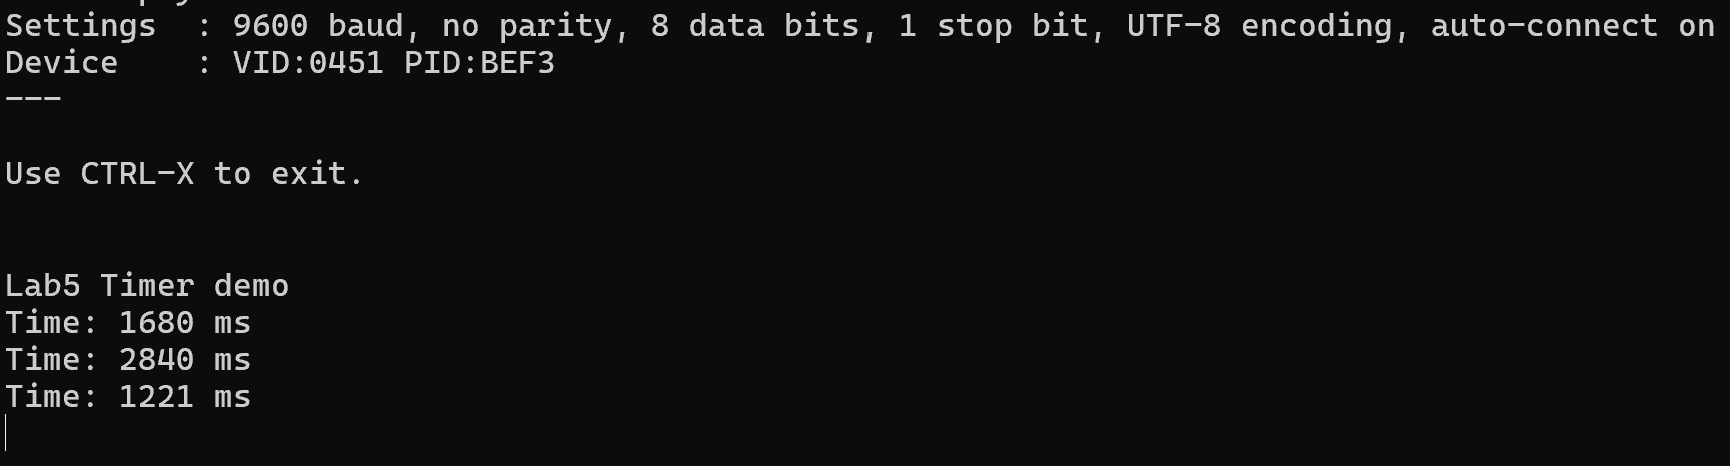
\includegraphics[width=\linewidth,decodearray={1 0 1 0 1 0}]{images/part1terminal.png}
    \caption{UART Output from Interrupt Testing}
    \label{part1terminal}
\end{figure}

These tests also confirmed that the port interrupts were functioning
correctly. The port interrupts were executed when the switches on the
MSP432 board were interracted with, allowing them to toggle the flashing
of the LED as well as telling the program when to start and stop the
counting of the 1kHz timer. Both of these functions were performed
successfully during these tests.

%end part 1

As a result of testing the circuit with various reflection distances, it was able to be
determined what an ideal testing distance would be, using both a 10k$\Omega$ and 20k$\Omega$ resistance. 
The results of these tests are shown in Table \ref{distanceVoltageCurrent}.

\begin{table}[H]
    \centering
    \caption{Phototransistor Voltage and Current at Various Distances}
    \label{distanceVoltageCurrent}
    \begin{tabular}{|c||c|c||c|c|}
        \hline
         & \multicolumn{2}{c||}{$R_{L1}$ = \textbf{10k}} & \multicolumn{2}{c|}{$R_{L1}$ = \textbf{20k}} \\
        \hline
        Distance & $V_{out}$ (V) & $IRL$ (mA) & $V_{out}$ (V) & $IRL$ (mA) \\
        \hline
        0 &  4.919 &  0.0081 & 4.810 & 0.0095 \\
        1 &  3.175 &  0.1820 & 1.225 & 0.1880 \\
        2 &  0.727 &  0.4261 & 0.737 & 0.2123 \\
        3 &  0.710 &  0.4278 & 0.698 & 0.2142 \\
        4 &  0.729 &  0.4259 & 0.683 & 0.2150 \\
        5 &  0.771 &  0.4217 & 0.687 & 0.2148 \\
        6 &  0.817 &  0.4171 & 0.697 & 0.2143 \\
        7 &  1.652 &  0.3339 & 0.716 & 0.2134 \\
        8 &  2.563 &  0.2430 & 0.735 & 0.2124 \\
        9 &  3.126 &  0.1869 & 0.751 & 0.2116 \\
        10 & 3.420 &  0.1576 & 0.765 & 0.2109 \\
        11 & 3.871 &  0.1126 & 0.790 & 0.2097 \\
        12 & 4.038 &  0.0959 & 0.806 & 0.2089 \\
        13 & 4.217 &  0.0781 & 0.820 & 0.2082 \\
        14 & 4.274 &  0.0724 & 0.880 & 0.2052 \\
        15 & 4.319 &  0.0679 & 1.346 & 0.1820 \\
        20 & 4.576 &  0.0423 & 3.430 & 0.0782 \\
        25 & 4.656 &  0.0343 & 4.078 & 0.0459 \\
        30 & 4.641 &  0.0358 & 4.243 & 0.0377 \\
        35 & 4.580 &  0.0419 & 4.200 & 0.0398 \\
        40 & 4.506 &  0.0493 & 4.043 & 0.0477 \\
        45 & 4.523 &  0.0476 & 4.018 & 0.0489 \\
        50 & 4.585 &  0.0414 & 4.082 & 0.0457 \\
        \hline
    \end{tabular}
\end{table}

Table \ref{distanceVoltageCurrent} demonstrates the relationship between the reflection distance
from the infrared diode to the phototransistor in the optoisolator, and the voltage and current across the
phototransistor. This relationship is slightly different when the circuit contains a 10k$\Omega$ resistor
and a 20k$\Omega$ resistor. The voltage relationships are shown more clearly in Fig.~\ref{distanceVoltageFigure}.

\subsection{Data Visualization and Analysis}

\begin{figure}[htbp]
    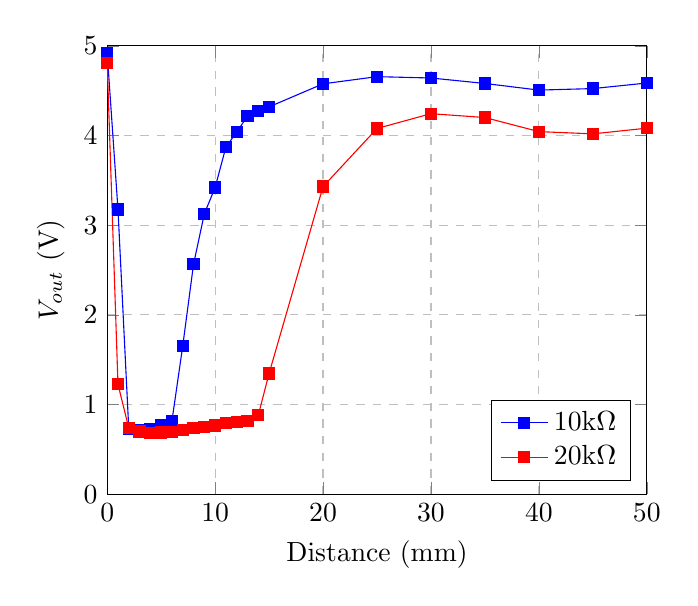
\begin{tikzpicture}
        \begin{axis} [
            xlabel={Distance (mm)},
            ylabel={$V_{out}$ (V)}, % might need to change this
            xmin=0, xmax=50,
            ymin=0, ymax=5,
            ymajorgrids=true,
            xmajorgrids=true,
            legend pos=south east,
            grid style=dashed,
        ]
            \addplot[
                color=blue,
                mark=square*
            ]
            coordinates {
                (0, 4.919)
                (1, 3.175)
                (2, 0.727)
                (3, 0.71)
                (4, 0.729)
                (5, 0.771)
                (6, 0.817)
                (7, 1.652)
                (8, 2.563)
                (9, 3.126)
                (10, 3.42)
                (11, 3.871)
                (12, 4.038)
                (13, 4.216)
                (14, 4.274)
                (15, 4.319)
                (20, 4.576)
                (25, 4.656)
                (30, 4.641)
                (35, 4.58)
                (40, 4.506)
                (45, 4.523)
                (50, 4.585)
            };
            \addlegendentry{10k$\Omega$}

            \addplot[
                color=red,
                mark=square*
            ]
            coordinates {
                (0, 4.81)
                (1, 1.225)
                (2, 0.7372)
                (3,0.6984)
                (4, 0.6831)
                (5, 0.6874)
                (6,0.6971)
                (7, 0.7156)
                (8, 0.735)
                (9, 0.7514)
                (10,0.765)
                (11, 0.7899)
                (12, 0.8059)
                (13, 0.82)
                (14, 0.8802)
                (15, 1.346)
                (20, 3.43)
                (25, 4.078)
                (30, 4.243)
                (35,4.2)
                (40, 4.043)
                (45, 4.018)
                (50, 4.0815)
            };
            \addlegendentry{20k$\Omega$}
        \end{axis}
    \end{tikzpicture}
    \caption{Distance of Reflective Surface from OPB745 vs Voltage}
    \label{distanceVoltageFigure}
\end{figure}

Fig.~\ref{distanceVoltageFigure} shows the voltage in both cases start at near the
logic high voltage and immediately drop, and then rise more
gradually back up to about 0.5 or 1.0 volts lower, for the
10k$\Omega$ case and 20k$\Omega$ case respectively. From these
voltage values, a current relationship could also be calculated
by subtracted $V_{out}$, that being the voltage across the
phototransistor, from the logic high voltage of 5 volts, which
gives the voltage across the resistor, and then using Ohm's law
to determine the current by dividing by the resistance. The
outcome of these calculations is shown in Fig.~\ref{distanceCurrentFigure}

\begin{figure}[htbp]
    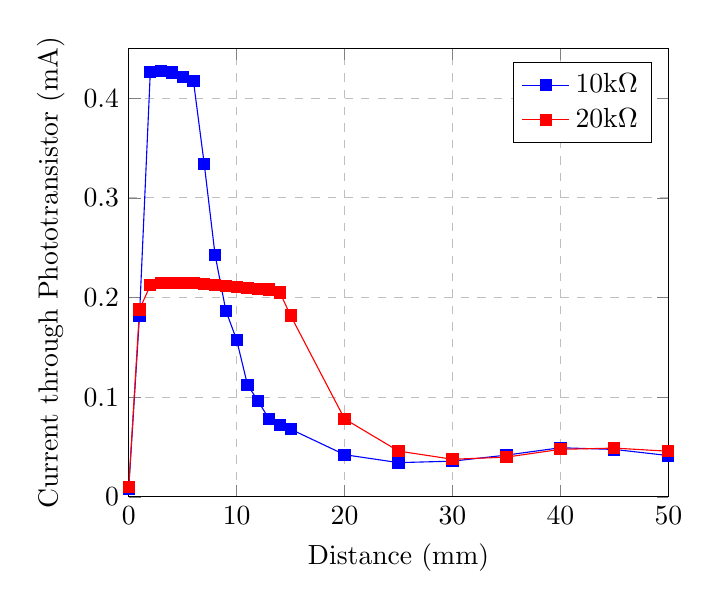
\begin{tikzpicture}
        \begin{axis} [
            xlabel={Distance (mm)},
            ylabel={Current through Phototransistor (mA)},
            xmin=0, xmax=50,
            ymin=0, ymax=0.45,
            ymajorgrids=true,
            xmajorgrids=true,
            legend pos=north east,
            grid style=dashed,
        ]
            \addplot[
                color=blue,
                mark=square*
            ]
            coordinates {
                (0,  0.008077383)
                (1,  0.181990427)
                (2,  0.426106901)
                (3,  0.427802154)                
                (4,  0.425907459)
                (5,  0.421719186)
                (6,  0.41713203 )
                (7,  0.333865178)
                (8,  0.243019545)
                (9,  0.186876745)
                (10, 0.157558835)                
                (11, 0.112584763)
                (12, 0.095931392)
                (13, 0.078111288)
                (14, 0.072397288)
                (15, 0.067909852)
                (20, 0.042281611)
                (25, 0.034303949)
                (30, 0.035799761)
                (35, 0.041882728)                
                (40, 0.049262066)
                (45, 0.047566813)
                (50, 0.041384124)
            };
            \addlegendentry{10k$\Omega$}

            \addplot[
                color=red,
                mark=square*
            ]
            coordinates {
                (0,  0.009462151)      
                (1,  0.187998008)       
                (2,  0.212290837)        
                (3,  0.214223108)        
                (4,  0.21498506 )        
                (5,  0.214770916)        
                (6,  0.214287849)        
                (7,  0.213366534)        
                (8,  0.212400398)       
                (9,  0.211583665)        
                (10, 0.210906375)       
                (11, 0.209666335)        
                (12, 0.208869522)        
                (13, 0.208167331)      
                (14, 0.205169323)        
                (15, 0.181972112)       
                (20, 0.078187251)      
                (25, 0.045916335)       
                (30, 0.037699203)       
                (35, 0.039840637)     
                (40, 0.047659363)       
                (45, 0.048904382)       
                (50, 0.045742032)        
            };
            \addlegendentry{20k$\Omega$}
        \end{axis}
    \end{tikzpicture}
    \caption{Distance of Reflective Surface from OPB745 vs Current}
    \label{distanceCurrentFigure}
\end{figure}

Fig.~\ref{distanceVoltageFigure} and Fig.~\ref{distanceCurrentFigure}
show the relationship between the distance of the reflective
material and the voltage and current associated with the
phototransistor in the OPB745. This data demonstrates three
stages within the relationship. 

When the voltage across the phototransistor is high and
the current through it is low, this means that the phototransistor is
less active, and a low voltage and higher current means
the phototransistor is more active. Therefore, in the first
stage, where the voltage is very high and the current is very
low, it is clear that the phototransistor is receiving almost
no light from the infrared diode. This is due to the fact
that the reflective coating is so close that the light from
the diode cannot escape the OPB745, leading to very little entering
the phototransistor.

In the next stage, the reflective material is far enough
from the OPB745 to allow light to exit, and due to the close
proximity, much is reflected directly into the phototransistor.
This causes the low voltage and high current seen in the data
after the dropoff from the first stage.

When the reflective material is moved far enough from the
device to allow reflected light to scatter to areas
other than the phototransistor, the voltage quickly rises and
the current falls. The values settle at a level that is
less extreme than the initial near-complete occlusion of
the phototransistor, as some light still reaches it.

\subsection{Comparison to Expectations}
The measured outputs of the circuit do not match fully with what was expected based upon
the datasheet of the OPB745. For visual comparison, data from Fig.~\ref{fig:expectedvoltage} and Fig.~\ref{distanceVoltageFigure}
are combined in Fig.~\ref{fig:expectedAndRealVoltage}.

\begin{figure}[htbp]
    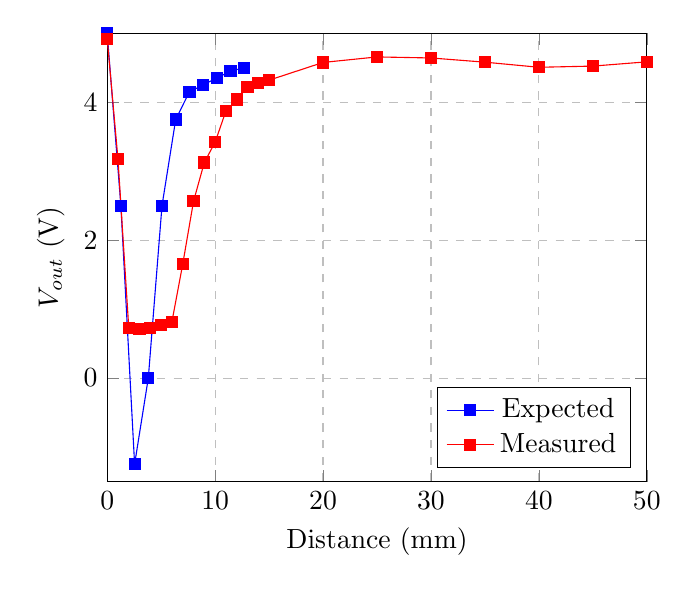
\begin{tikzpicture}
        \begin{axis} [
            xlabel={Distance (mm)},
            ylabel={$V_{out}$ (V)}, % might need to change this
            xmin=0, xmax=50,
            ymin=-1.5, ymax=5,
            ymajorgrids=true,
            xmajorgrids=true,
            legend pos=south east,
            grid style=dashed,
        ]
            \addplot[
                color=blue,
                mark=square*
            ]
            coordinates {
                (0, 5)
                (1.27, 2.5)
                (2.54, -1.25)
                (3.81, 0)
                (5.08, 2.5)
                (6.35, 3.75)
                (7.62, 4.15)
                (8.89, 4.25)
                (10.16, 4.35)
                (11.43, 4.45)
                (12.7, 4.5)
            };
            \addlegendentry{Expected}

            \addplot[
                color=red,
                mark=square*
            ]
            coordinates {
                (0, 4.919)
                (1, 3.175)
                (2, 0.727)
                (3, 0.71)
                (4, 0.729)
                (5, 0.771)
                (6, 0.817)
                (7, 1.652)
                (8, 2.563)
                (9, 3.126)
                (10, 3.42)
                (11, 3.871)
                (12, 4.038)
                (13, 4.216)
                (14, 4.274)
                (15, 4.319)
                (20, 4.576)
                (25, 4.656)
                (30, 4.641)
                (35, 4.58)
                (40, 4.506)
                (45, 4.523)
                (50, 4.585)
            };
            \addlegendentry{Measured}
        \end{axis}
    \end{tikzpicture}
    \caption{Measured and Expected Output Voltages of OPB745}
    \label{fig:expectedAndRealVoltage}
\end{figure}

Fig.~\ref{fig:expectedAndRealVoltage} provides a visual comparison between the measured and expected
outputs of the OPB745 at varying distances from a reflective surface, and demonstrates that there is
a sizable difference between them. There are two primary differences between the graphs, both relating to
the area where most light is reflected. In the expected data, the dip falls to a negative voltage across
the phototransistor, whereas in the measured data, the output voltage only falls to about 0.7 volts. This is
due to the fact that in ideal circumstances, the phototransistor would flow enough current that the voltage
drop across the resistor is greater than 5 volts, leading to a negative current across the phototransistor.
In the real world circuit, loss of light and possible current limiting causes the voltage to stop decreasing before
crossing zero.

The other major difference is the difference in range over which this voltage drop occurs. The OPB745 datasheet
assumes a flat reflective surface, however the aluminum foil used in this setup has a slightly altered affect.
This may be due to a slightly convex circuit allowing a greater range of distances to reflect light in the
correct spot. Although it appears that the bottom of the voltage drop has a flat response over this section
from approximately 2mm to 6mm, it may be that the voltage would have gone lower and was only stopped by
the phototransistor's physical characteristics, and so does not necessarily imply a steady amount of light
received by the phototransistor.

\subsection{Usage with Digital Logic}

In order for the OPB745 to be used as an isolator in a digital
circuit, the output must be interpreted as a digital signal.
This was done by passing the output through an 74LS14 
Schmitt-trigger inverter, as
well as feeding the input diode with the output of an 7406
inverter. In steady state with working components, this circuit
will behave as intended. However, due to the partially analog
nature of the circuit, there is a switching frequency where
this correct digital behavior begins to break down. The circuit
was fed with a switching signal with both the input and output voltage
monitored by a oscilloscope. The maximum operable frequencies using
10k$\Omega$ and 20k$\Omega$ resistors were
recorded in their working state and shown in Fig.~\ref{fig:maxFreq10k} and Fig.~\ref{fig:maxFreq20k} respectively.

\begin{figure}[!ht]
    \centering
    % 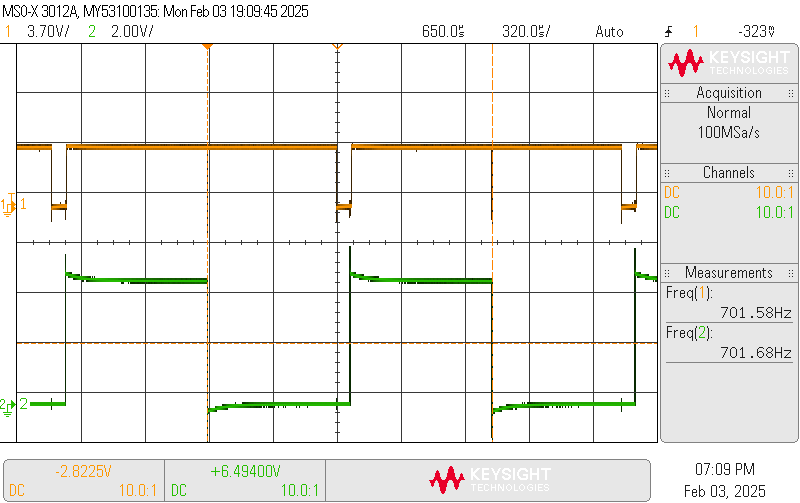
\includegraphics[width=\linewidth]{images/10k Before Good.png}
    \caption{\textit{Maximum Switchable Frequency with 10k$\Omega$ Resistor}}
    \label{fig:maxFreq10k}
\end{figure}

\begin{figure}[!ht]
    \centering
    % 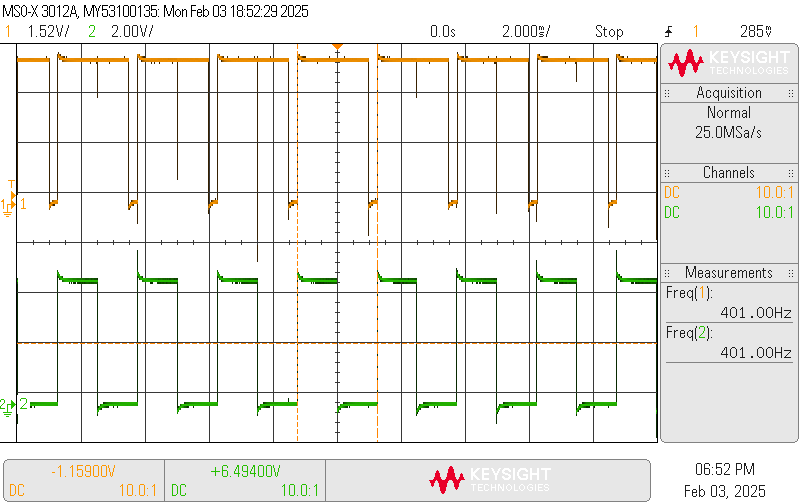
\includegraphics[width=\linewidth]{images/20k Before.png}
    \caption{\textit{Maximum Switchable Frequency with 20k$\Omega$ Resistor}}
    \label{fig:maxFreq20k}
\end{figure}

Fig.~\ref{fig:maxFreq10k} demonstrates that the circuit with the 10k$\Omega$
resistor operated at a maximum frequency of about 700Hz, while Fig.~\ref{fig:maxFreq20k}
demonstrates that the circuit with the 20k$\Omega$ resistor could operate at only 400Hz.

\section{Questions}

\subsection{In the lab we do not use a 7406 inverter on the output; instead we use the 74LS14 with Schmitt
trigger. Why do we need to do this, and what is the difference between the two?}

We need to use the 74LS14 to provide additional protection against noise on the output, as it
prevents multiple edges from being produced from a signal crossing a threshold voltage. It does this
by switching to high and low outputs at diffenent input voltages, leaving something like a voltage dead-zone,
where changes in voltage up or down will only affect the output after reaching a certain point past the middle
of the voltage range. This dead-zone is refered to as the hysteresis region. The 7406 is not a Schmitt trigger
and does not have a hysteresis region, only a single threshold voltage, making the output voltages entirely
defined by the current input.

\subsection{Why does the voltage start at ~5V at 0mm and then drop quickly? Why does it eventually go
back to ~5V?}

The voltage starts at about 5V due to the fact that the
phototransistor is nearly completely off at 0mm. This is
because when the reflective material is fully pressed against
the OPB745, it blocks both the infrared diode from emitting
light outside the device, and blocks the phototransistor from
receiving any light. Once the material is moved back a small amount, the
infrared light can be reflected most effectively to the
phototransistor, turning it on and decreasing the voltage
across it. When the material continues to be moved further 
back, a point is crossed where the light begins to be scattered
to other locations and becomes less focused on the
phototransistor, leading the phototransistor to turn on less,
flowing less current, and therefore for the voltage over the
component to gradually increase.

\subsection{Why does the frequency change when going from a 10k$\Omega$ load resistor to a 20k$\Omega$ load resistor?
Did you anticipate it increasing or decreasing and why?}

When doubling the size of the load resistor from 10k$\Omega$  to 20k$\Omega$, the frequency changes because the transistor is recieving
less voltage as more is being lost across the resistor. As a result of the lower voltage, the transistor has less range to decipher
whether the incoming signal is high or low on the square wave. With more voltage, faster frequencies are less damaging to the results as
the actual signal can still be detected. It is expected, therefore, that the circuit with the 20k$\Omega$ load resistor will break down
at a slower frequency than the circuit with the 10k$\Omega$ is able to achieve.

\section{Conclusion}
Through the course of this exercise, the properties of the OPB745 were shown and its behavior was compared between a laboratory
setting and the expected values shown on the datasheet. Because the measured results of the tests showed similar characteristics and
patterns to that of the datasheet's values, the exercise can be deemed a success. In the future, the OPB745 can be used to detect changes
in an environment without requiring contact, something which will be immensely helpful in developing autonomous car technology. It was
necessary, however, to understand how the device functions before it could be put to use in more specialized applications.

\end{document}
